\begin{flushright} {\tiny {\color{gray} benchmark\_sscb3D.tex}} \end{flushright}
%~~~~~~~~~~~~~~~~~~~~~~~~~~~~~~~~~~~~~~~~~~~~~~~~~~~~~~~~~~~~~~~~~~~~~~~~~~~~~~~~~~~~~~~~~~~~~~~~~~


The governing equations are those of an incompressible fluid with constant viscosity whose 
density depends on temperature. The fluid convects in a three-dimensional hollow sphere. 
The inner radius is 11/9 while the outer radius is 20/9, so that the depth of the mantle is exactly 1.
Boundary conditions are free-slip at the top
and bottom boundaries and isothermal with nondi-
mensional temperatures of 0 and 1 at the top and
bottom boundaries, respectively.

The dynamics of the system are gouverned by the Rayleigh number:
\[
\Ranb=\frac{\rho_0 \alpha g \; \Delta T \; \Delta R^3 }{\kappa \eta}
\]
Initial conditions for temperature are given as a function
of coordinates with perturbations at some given
spherical harmonics superimposed on a conductive
temperature profile:

\[
T(r,\theta,\phi)
=\frac{R_i(r-R_o)}{r(R_i-R_o)} 
+
\sum_m
\left[
\epsilon_{c,m} \cos m\phi + \epsilon_{s,m} \sin m\phi
\right]
p_{lm}(\theta) \sin\left( \pi \frac{r-R_i}{R_o-R_i}  \right)
\]
The first term represents a purely conductive temperature profile, while the second term 
is a perturbation to this profile, determining the final patterns of polyhedral symmetry. 
$l$ and $m$ are the spherical harmonic degree and order, respectively.
$\epsilon_{c,m}$ and $\epsilon_{s,m}$ are the magnitudes of the
individual spherical harmonic constituents.
$p_{lm}$ is a normalized associated Legendre
polynomial that is related to the associated
Legendre polynomial $P_{lm}$ as\footnote{There is a typo in \cite{shpe15}}:
\[
p_{lm}(\theta) 
= \sqrt{ \frac{(2l+1)(l-m)!}{2\pi (1+\delta_{m0})(l+m)!}  } P_l^m(\theta) 
\]
where $P_l^m$ are the (unnormalized) associated Legendre functions and  $\delta_{m0}$ 
is the Kronecker delta.

Note that there are somewhat subtle notation differences between the 
papers reporting on this benchmark with regards to the spherical 
harmonic parts and the normalisation term. 
Also note that the $(1+\delta_{m0})$ term is often omitted from 
spherical harmonics libraries (see \aspect documentation). 

%$Y_l^m$ denotes the normalized spherical harmonic of degree $l$ and order $m$ and the 
%nonaxisymmetric perturbation $\epsilon$ will play an important role in studying transitional 
%pattern formations in the cubic case.

%\[
%Y_l^m(\theta,\phi) = \sqrt{ \frac{(2l+1)(l-m)!}{2\pi (1+\delta_{m0})(l+m)!}  } P_l^m(\cos\theta) \cos (m\phi)
%\]

%The first is axisymmetric, the second is not.

In each case, we compute, as a function of time, Nusselt 
numbers for both the top and bottom boundaries, $Nu_t$ and $Nu_b$, 
averaged temperature for
the whole mantle, $<T>$ and averaged RMS velocity $v_{rms}$ for the whole mantle
with
\[
Nu_t=\frac{R_o(R_o-R_i)}{R_i} Q_t
\quad\quad
Nu_b=\frac{R_i(R_o-R_i)}{R_o} Q_b
\]
where $Q_t$ and $Q_b$ are the surface and bottom heat fluxes.

\begin{center}
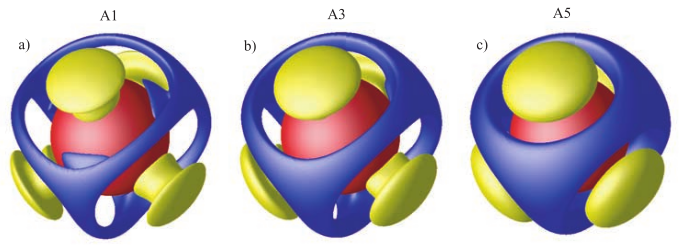
\includegraphics[width=10cm]{images/benchmark_sscb3D/zhmt08}\\
{\captionfont Taken from Zhong \etal (2008) \cite{zhmt08}. 
Representative steady state residual temperature 
$\delta T = T(r,\theta,\phi)-\langle T(r) \rangle$ for cases a, b, c.}
\end{center}


\Literature: Zhong \etal \cite{zhmt08} (\citcoms), Arrial \etal \cite{arfw14}
(\citcoms vs. radial basis function), Shahnas \etal \cite{shpe15} (own code), 
Liu \& King \cite{liki19} (\aspect).





